\documentclass[14pt, a4paper]{scrartcl}
\usepackage[utf8]{inputenc}
\usepackage[english,russian]{babel}
\usepackage{indentfirst}
\usepackage{misccorr}
\usepackage{graphicx}
\usepackage{amsmath}
\usepackage[utf8]{inputenc}
\usepackage[T1]{fontenc}
\usepackage{float}
\title{Определение систематических и случайных погрешностей при измерении удельного сопротивления нихромовой проволоки}
\author{Кирилл Балбек Б06-801}
\date{19.09.2018}

\usepackage{natbib}
\usepackage{graphicx}

\begin{document}
\maketitle

\section{Введение}
\subsection{Название}
Определение систематических и случайных погрешностей при измерении удельного сопротивления нихромовой проволоки
\subsection{Номер}
1.1.1
\subsection{Цели}
Измерить удельное сопротивление проволоки и вычислить систематические и случайные погрешности при использовании таких измерительных приборов, как линейка, штангенциркуль, микрометр, амперметр, вольтметр и мост постоянного тока.
\subsection{Задачи}
\paragraph{}
1. Ознакомиться с устройством и работой измерительных инструментов и приборов.
\paragraph{}
2. Измерить диаметр проволоки на 8-10 различных участках и запишите измерения в таблицу. Сравнить результаты, полученные при измерении микрометром и штангенциркулем. Усреднить полученные значения диаметра. Рассчитать площадь поперечного сечения проволоки, оценить погршность результата.
\paragraph{}
3. Составить таблицу основных характеристик амперметра и вольтметра: система прибора, класс точности, предел измерений $x_n$, число делений шкалы $n$, цена делений $x_n/n$, чувствительность $n/x_n$, абсолютная погрешность $\Delta x_M$, внутреннее сопротивление прибора (на данном пределе измерений).
\paragraph{}
4. Используя значения внутренних сопротивлений, указанных на приборах, и зная, что сопротивление проволоки по порядку величины равно 5 Ом, оценить величину поправок при измерениях $R_\text{пр}$ по схемам рис. 1. Для работы выбрать ту из схем, которая приводит к меньшей поправке.
\paragraph{}
5. Измерьте с помощью линейки длину исследуемого участка проволоки (между подвижным и неподвижным прижимными контактами) и собрать выбранную электрическую схему. Включить ток. Изменяя его с помощью реостата, записать в виде таблицы показания амперметра и вольтметра в 10 точках. Провести измерения при возрастающих и убывающих значениях тока. Построить график зависимости $V = f(I)$ и с его помощью рассчитать измеренную величину сопротивления R, а затем вычислить искомое $R_\text{пр}$. Оценить, с какой ошибкой найдена величина $R_\text{пр}$.
\paragraph{}
6. Измерить искомое сопротивление проволоки с помощью моста P4833. 
\paragraph{}
7. Провести измерения по пп. 5, 6 для трех различных длин проволоки.
\paragraph{}
8. Определить удельное сопротивление проволоки. Оценить допущенную при этом погрешность.
\paragraph{}
9. Сравнить полученные результаты с табличными значениями.
\subsection{Оборудование и экспериментальная установка}
Линейка, штангенциркуль, микрометр, отрезок проволоки из нихрома, амперметр, вольтметр, источник ЭДС, мост постоянного тока, реостат, ключ.
\begin{figure}
\centering
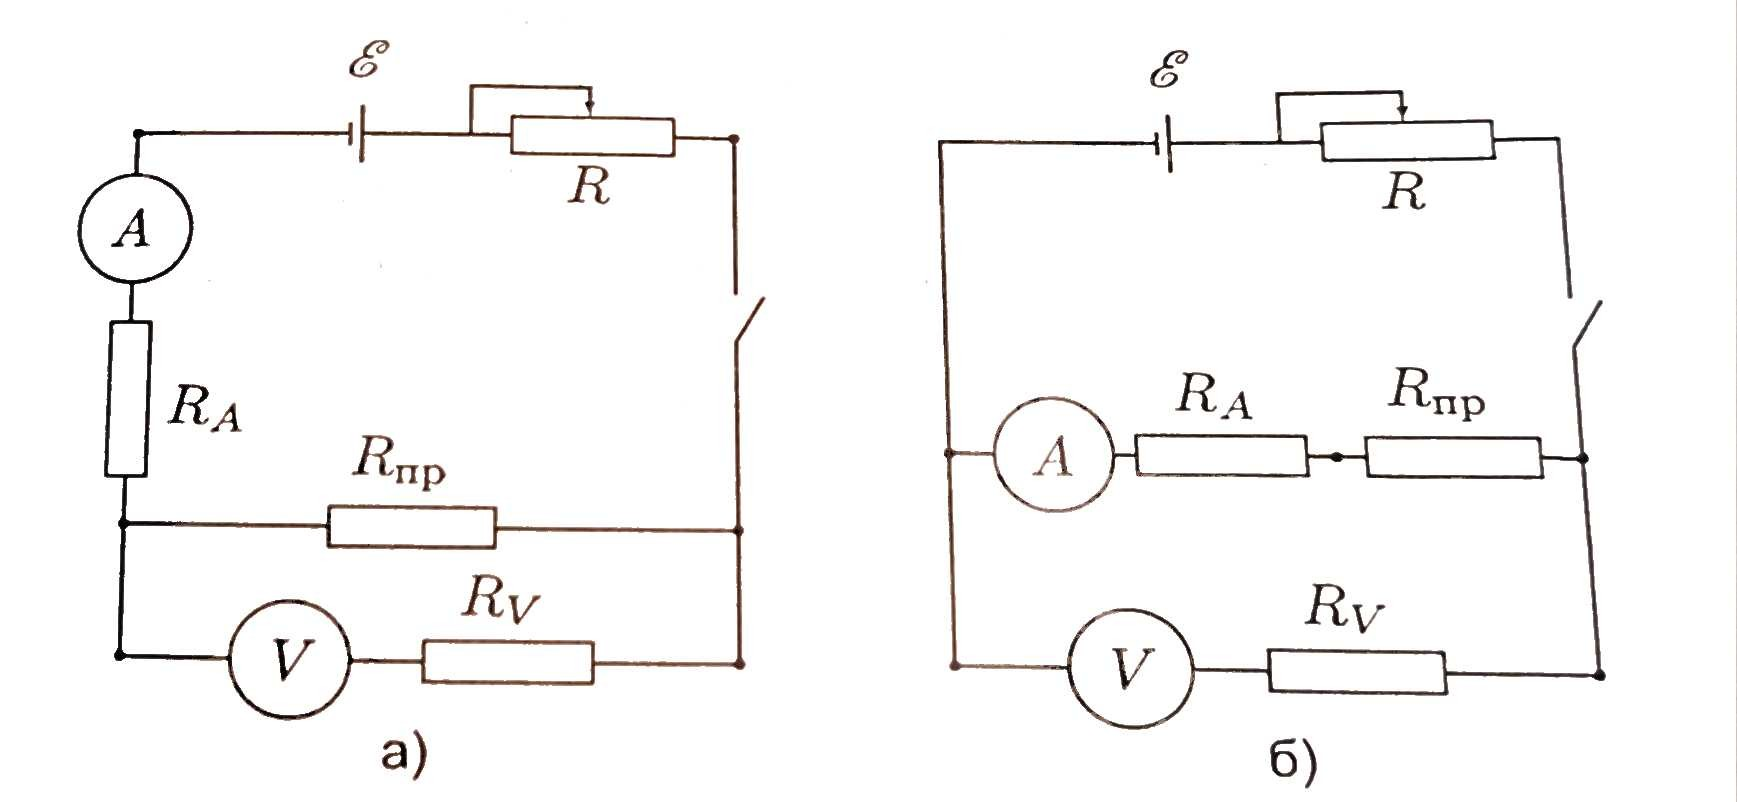
\includegraphics[scale=0.2]{12schemes.jpg}
\caption{Схемы для измерения сопротивления при помощи амперметра и вольтметра}
\label{fig:scheme12}
\end{figure}

\section{Основная часть}
\subsection{Теоретическая справка}
\paragraph{}
 Для схемы а) (рис. 1) сопротивление будет считаться по формуле:
\begin{equation}
R_\text{пр1}=  \frac{V_\text{а}}{I_\text{а}}=R_\text{пр}\frac{R_v}{R_\text{пр}+R_v}\approx R_\text{пр1}(1+\frac{R_\text{пр1}}{R_v})
\end{equation}
\paragraph{}
Для схемы б) (рис.1) споротивление будет считаться по формуле:
\begin{equation}
R_\text{пр2}=  \frac{V_\text{б}}{I_\text{б}}=R_\text{пр}+R_A=R_\text{пр2}(1-\frac{R_A}{R_\text{пр2}})
\end{equation}
\subsection{Методика измерений}

\paragraph{}
1. Точность измерения с помощью штангенциркуля - 0,1 мм. Точность измерения с помощью микрометра - 0,01 мм.
\paragraph{}
2. Измеряем диаметр проволоки штангенциркулем ($d_1$) и микрометром ($d_2$) на 10 различных участках:

\begin{table}[H]
\caption{\label{tab:diametr}Результаты измерения диаметра проволоки.}
\begin{center}
\begin{tabular}{|c|c|c|c|c|c|c|c|c|c|c|}
\hline
& 1 & 2 & 3 & 4 & 5 & 6 & 7 & 8 & 9 & 10 \\
\hline
$d_1$, мм & 0,4 & 0,4 & 0,4 & 0,4 & 0,4 & 0,4 & 0,4 & 0,4 & 0,4 & 0,4  \\
\hline
$d_2$, мм & 0,36 & 0,36 & 0,37 & 0,39 & 0,36 & 0,36 & 0,36 & 0,37 & 0,36 & 0,36  \\
\hline
\multicolumn{11}{|c|}{$\overline{d_1} = 0,4$ мм; $\overline{d_2} =  0,366$ мм} \\
\hline
\end{tabular}
\end{center}
\end{table} 
\paragraph{}
При измерении диаметра проволоки штангенциркулем случайная погрешность отсутствует. Следовательно, точность результата определяется только точностью штангенциркуля (систематической погрешностью):
\begin{equation}\label{eq:d1}
d_1 = (0,4 \pm 0,1), 
\end{equation}

\paragraph{}
Измерения с помощью микрометра содержат как систематическую, так и случайную погрешности:

\begin{equation}\label{eq:sigmasist}
\sigma_\text{сл}=0,01 \text{ мм}, 
\end{equation}

\begin{equation}\label{eq:sigmasled}
\sigma_\text{сист}=\frac1N\sqrt{\sum_{i=1}^n (d-\overline{d})^2}=\frac{1}{10}\sqrt{8,4\cdot10^{-4}}\approx2,9\cdot10^{-3} \text{мм},
\end{equation}


\begin{equation}\label{eq:sigmasist}
\sigma=\sqrt{\sigma_\text{сист}^2+\sigma_\text{сл}^2}=\sqrt{(0,01)^2+(0,0029)^2}\approx0,01 \text{мм}, 
\end{equation}

Поскольку $\sigma_\text{сист}^2\gg\sigma_\text{сл}^2$, проволоку можно считать однородной по диаметру, а погрешность диаметра $\sigma_ d$ определяется только $\sigma_\text{сист}$ микрометра:

\begin{equation}\label{eq:d2powtor}
d_2=\overline{d_2}\pm\sigma_d=(0,366\pm0,010)\text{мм}=(3,66\pm0,10)\cdot10^{-2} \text{см}
\end{equation}


\paragraph{}
3. Определим площадь поеречного сечения проволоки:
\begin{equation}\label{eq:Splochad}
S=\frac{\pi d_2^2}{4} = \frac{3,14\cdot(3,66\cdot10^{-2})}{4}\approx1,05\cdot10^{-3} \text{см}^2
\end{equation}
\paragraph{}
Найдем величину погрешности $\sigma_s$:
\begin{equation}\label{eq:Splochad2}
\sigma_S=2\frac{\sigma_d}{d}S = 2\cdot\frac{0,01}{0,37}\cdot1,05\cdot10^{-3}=5,68\cdot10^{-5}\text{см}^2
\end{equation}
\paragraph{}
Итак, $S=(1,05\pm0,06)\cdot10^{-3}\text{см}^2$,т.е. площадь поперечного сечения проволоки определена с точнстью 6\%.

\paragraph{}
4. Сведем основные характеристики приборов в таблицу 2.

\begin{table}[H]
\caption{\label{tab:charast}Основные характеристики приборов.}
\begin{center}
\begin{tabular}{|c|c|c|}
\hline
& Вольтметр & Амперметр \\
\hline
Система&Цифровой&Магнитоэлектрический\\
Класс точности&Цифровой&0,5\\
Предел измерений $x_n$& Цифровой & 300 мА\\
Число делений шкалы $n$& Цифровой & 150\\
Цена делений $x_n/n$& Цифровой & 2мА/дел\\
Чувствительность $n/x_n$& Цифровой & 0,5 дел/мА\\
Абсолютная погрешность $\Delta x_M$ & Цифровой & 1,5 мА\\
Внутреннее сопротивление прибора & 10МОм & 0,32 Ом\\
\hline
\end{tabular}
\end{center}
\end{table} 

\paragraph{}
5.Известно, что $R_\text{пр}\approx 5$ Ом, $R_v=500$ Ом, $R_A = 1$ Ом. Оценим по формулам (1) и (2) величину поправок при измерении $R_\text{пр}$:
\paragraph{}
Для схемы рис. 1а $\frac{5}{500}=0,01$, т.е. 1\%
\paragraph{}
для схемы рис. 1а $\frac{1}{5}=0,2$, т.е. 20\%
\paragraph{}
Вывод: при измерении относительно небольших сопротивлений меньшую ошибку дает схема рис. 1а.
\paragraph{}
6. Собираем схему рис. 1а.
\paragraph{}
Опыт проводим для 4 длин проволоки: ($10,0\pm0,1$) см, ($20,0\pm0,1$) см, ($30,0\pm0,1$) см, ($50,0\pm0,1$) см. Показания приборов запишем в таблицу 3. Результаты измерения с помощью моста P4833 заносим в таблиу 4.
\paragraph{}
 8.  Строим графики при помощи зависимостей $V=f(I)$ для всех четверых отрезков проволоки, проводя прямые через экспериментальные точки (рис. 2, 3, 4, 5). Из графиков видно, что нет различия между значениями, полученными при возрастании и при уменьшении тока.
 \paragraph{}
 9. Для каждой длины l расчет проводим методов наименьших квадратов для прямой, проходящей через начало координат. Сопротивление находим как: $R_\text{ср}=\frac{<VI>}{I^2}$, среднеквадратичную случайную ошибку как: $\sigma_\text{Rcp}^\text{сист}=\frac{1}{\sqrt{10}}\sqrt{\frac{<V^2>}{<I^2>}-R_\text{cp}^{2}}$, где 10 - число экспериментальных точек для каждого l. Результаты запишем в таблицу 4.
 \paragraph{}
 10.Возможную систематическую погрешность $R_cp$ оцениваем по формуле:

 $\frac{\sigma_\text{Rcp}^\text{сист}}{R_cp}=\sqrt{(\frac{\sigma_V}{V})^2+(\frac{\sigma_I}{I})^2}$
 
 \paragraph{}
 
\begin{table}[H]
\caption{\label{tab:voltmeterampermeter}Показания вольтметра и амперметра.}
\begin{center}
\begin{tabular}{|c|c|c||c|c|c||c|c|c||c|c|c|}
\hline
\multicolumn{3}{|c|}{$l=10$ см}& \multicolumn{3}{|c|}{$l=20$ см} & \multicolumn{3}{|c|}{$l=30$ см} & \multicolumn{3}{|c|}{$l=50$ см}\\
\hline
$I$,&$V$,&$I$ & $I$,&$V$,&$I$, & $I$,&$V$,&$I$, & $I$,&$V$,&$I$,\\
дел, & мВ, & мА $\cdot$ & дел, & мВ, & мА $\cdot$ & дел, & мВ, & мА $\cdot$& дел, & мВ, & мА $\cdot$\\
$0,5_\text{дел}^\text{мА}$&&$\cdot10^{-1}$&$0,5_\text{дел}^\text{мА}$&&$\cdot10^{-1}$&$0,5_\text{дел}^\text{мА}$&&$\cdot10^{-1}$&$0,5_\text{дел}^\text{мА}$&&$\cdot10^{-1}$\\
\hline
34&17,6&170& 50&51&250& 44&68&220& 20&51,1&100\\
\hline
41&21,4&190& 54&54,8&270& 45&69,3&225& 22&56&110\\
\hline
60,5&30,8&205& 64&64,7&320& 51&78&255& 29&76&145\\
\hline
75,5&38,8&240& 71&72,5&355& 52&79&260& 39&101,7&195\\
\hline
101&52,3&302,5& 82&83,8&410& 64&98&320& 54&141&270\\
\hline
95&48,7&305& 105&107&525& 69&106&345& 34&88&170\\
\hline
82&42&377,5& 82&84,5&410& 75&115&375& 39&103&195\\
\hline
61&31,3&410& 71&71&355& 33&51&165& 48&124&240\\
\hline
48&25&475& 62&63,5&310& 33&57,4&165& 21&53,4&105\\
\hline
38&20&505 &48&48,7&240& 54&82,9&270& 25&65&125\\
\hline

\end{tabular}
\end{center}
\end{table}

\paragraph{}

\begin{table}[H]
\caption{\label{tab:soprot}Результаты измерения сопротивления проволоки.}
\begin{center}
\begin{tabular}{|c||c||c||c||c|}
\hline
&$l=10$ см & $l=20$ см & $l=30$ см & $l=50$ см \\
\hline
$R_0$ (\text{По P4833}), \text{Ом}&1,064 & 2,08& 3,097 & 5,226\\
$R_\text{cp}$, \text{Ом}&1,03 & 2,04& 3,11 & 5,18\\
$R_\text{пp}$, \text{Ом}&1,030000011 & 2,040000042& 3,110000097 & 5,180000268\\
$\sigma_\text{R}^ \text{случ}$, \text{Ом}&0,00256 & 0,00273& 0,0129 & 0,014954\\
$\sigma_\text{R}^ \text{сист}$, \text{Ом}&0,000457506743 & 0,0008636438577& 0,00173727655 & 0,004447448908\\
\hline
\end{tabular}
\end{center}
\end{table} 

\begin{figure}
\centering
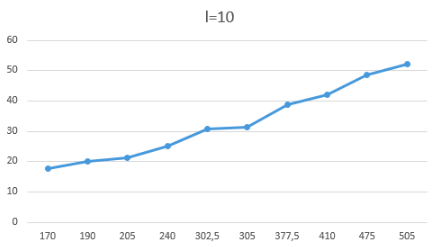
\includegraphics[scale=1]{leq10.png}
\caption{График l = 10}
\label{fig:10len}
\end{figure}
\begin{figure}
\centering
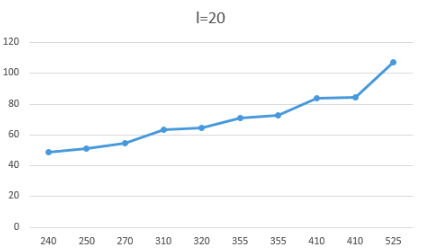
\includegraphics[scale=1]{leq20.png}
\caption{График l = 20}
\label{fig:20len}
\end{figure}
\begin{figure}
\centering
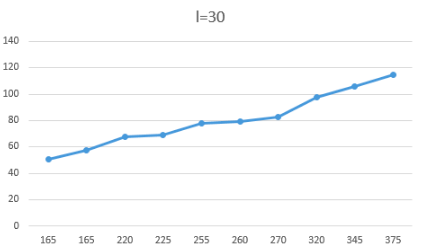
\includegraphics[scale=1]{leq30.png}
\caption{График l = 30}
\label{fig:30len}
\end{figure}
\begin{figure}
\centering
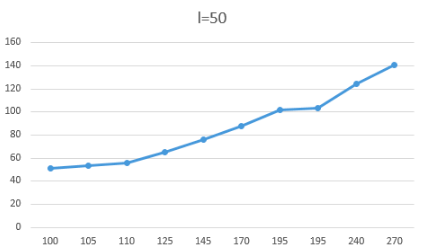
\includegraphics[scale=1]{leq50.png}
\caption{График l = 50}
\label{fig:50len}
\end{figure}

\begin{table}[H]
\caption{\label{tab:charast}Основные характеристики приборов.}
\begin{center}
\begin{tabular}{|c|c|c|c|c|}
\hline
l, см& 10 & 20 & 30 & 50 \\
\hline
$R_\text{cp}$,Ом & &  & &\\
\hline
$\sigma_R$, Ом & & & &\\
\hline
\end{tabular}
\end{center}
\end{table} 

\section{Conclusion}
``I always thought something was fundamentally wrong with the universe'' \citep{adams1995hitchhiker}

\bibliographystyle{plain}
\bibliography{references}
\end{document}
